%% Source of figures/empirical-tuning.pdf. Compile: pdflatex empirical-tuning.tex
%% Generated 2026-10-28 from the SMOTE25 evaluation draft page (76 coded papers, 71 empirical).
%% Numbers are filled from the coded data; regenerate instead of editing them by hand.
\documentclass[border=4pt]{standalone}
\usepackage[scaled]{helvet}\renewcommand{\familydefault}{\sfdefault}
\usepackage{pgfplots}\pgfplotsset{compat=1.18}
\definecolor{sOne}{HTML}{2A78D6}\definecolor{sTwo}{HTML}{EB6834}\definecolor{sThree}{HTML}{1BAF7A}\definecolor{sFour}{HTML}{EDA100}
\definecolor{oZero}{HTML}{A3ABB4}\definecolor{oOne}{HTML}{5598E7}\definecolor{oTwo}{HTML}{1C5CAB}\definecolor{oThree}{HTML}{0D366B}\definecolor{inkTwo}{HTML}{465462}
\begin{document}
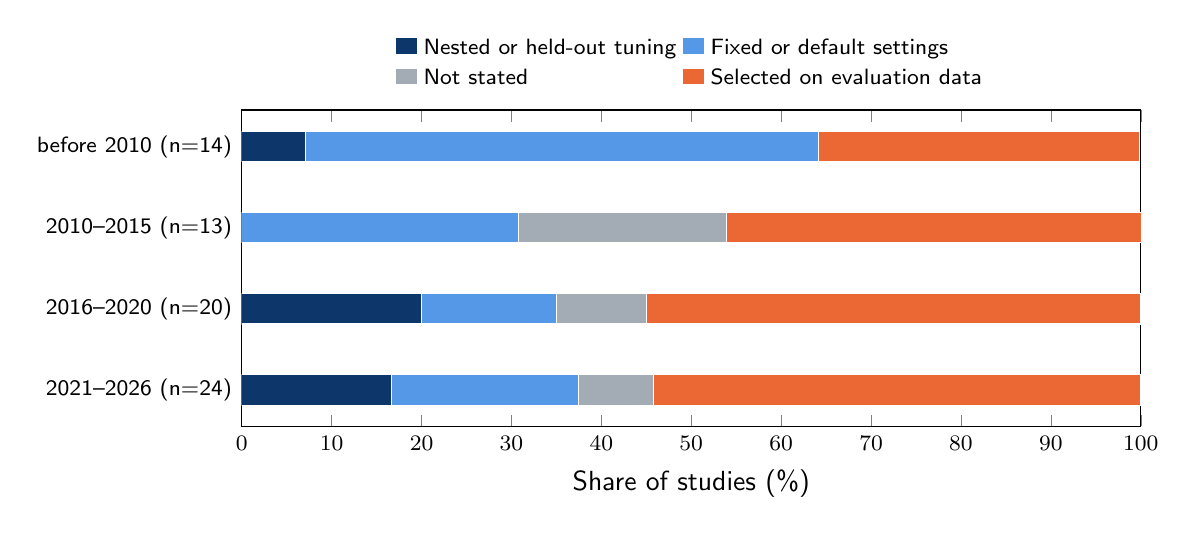
\begin{tikzpicture}
\begin{axis}[xbar stacked,width=13cm,height=5.6cm,bar width=11pt,xmin=0,xmax=100,y dir=reverse,ytick={0,...,3},
  yticklabels={{before 2010 (n=14)},{2010--2015 (n=13)},{2016--2020 (n=20)},{2021--2026 (n=24)}},xlabel={Share of studies (\%)},enlarge y limits=0.15,
  tick label style={font=\footnotesize},legend cell align=left,legend style={font=\footnotesize,at={(0.5,1.03)},anchor=south,legend columns=2,draw=none}]
\addplot[fill=oThree,draw=white] coordinates {(7.1,0) (0.0,1) (20.0,2) (16.7,3)};
\addplot[fill=oOne,draw=white] coordinates {(57.1,0) (30.8,1) (15.0,2) (20.8,3)};
\addplot[fill=oZero,draw=white] coordinates {(0.0,0) (23.1,1) (10.0,2) (8.3,3)};
\addplot[fill=sTwo,draw=white] coordinates {(35.7,0) (46.2,1) (55.0,2) (54.2,3)};
\legend{{Nested or held-out tuning},{Fixed or default settings},{Not stated},{Selected on evaluation data}}
\end{axis}
\end{tikzpicture}
\end{document}
